\begin{figure*}[!t]
\centering
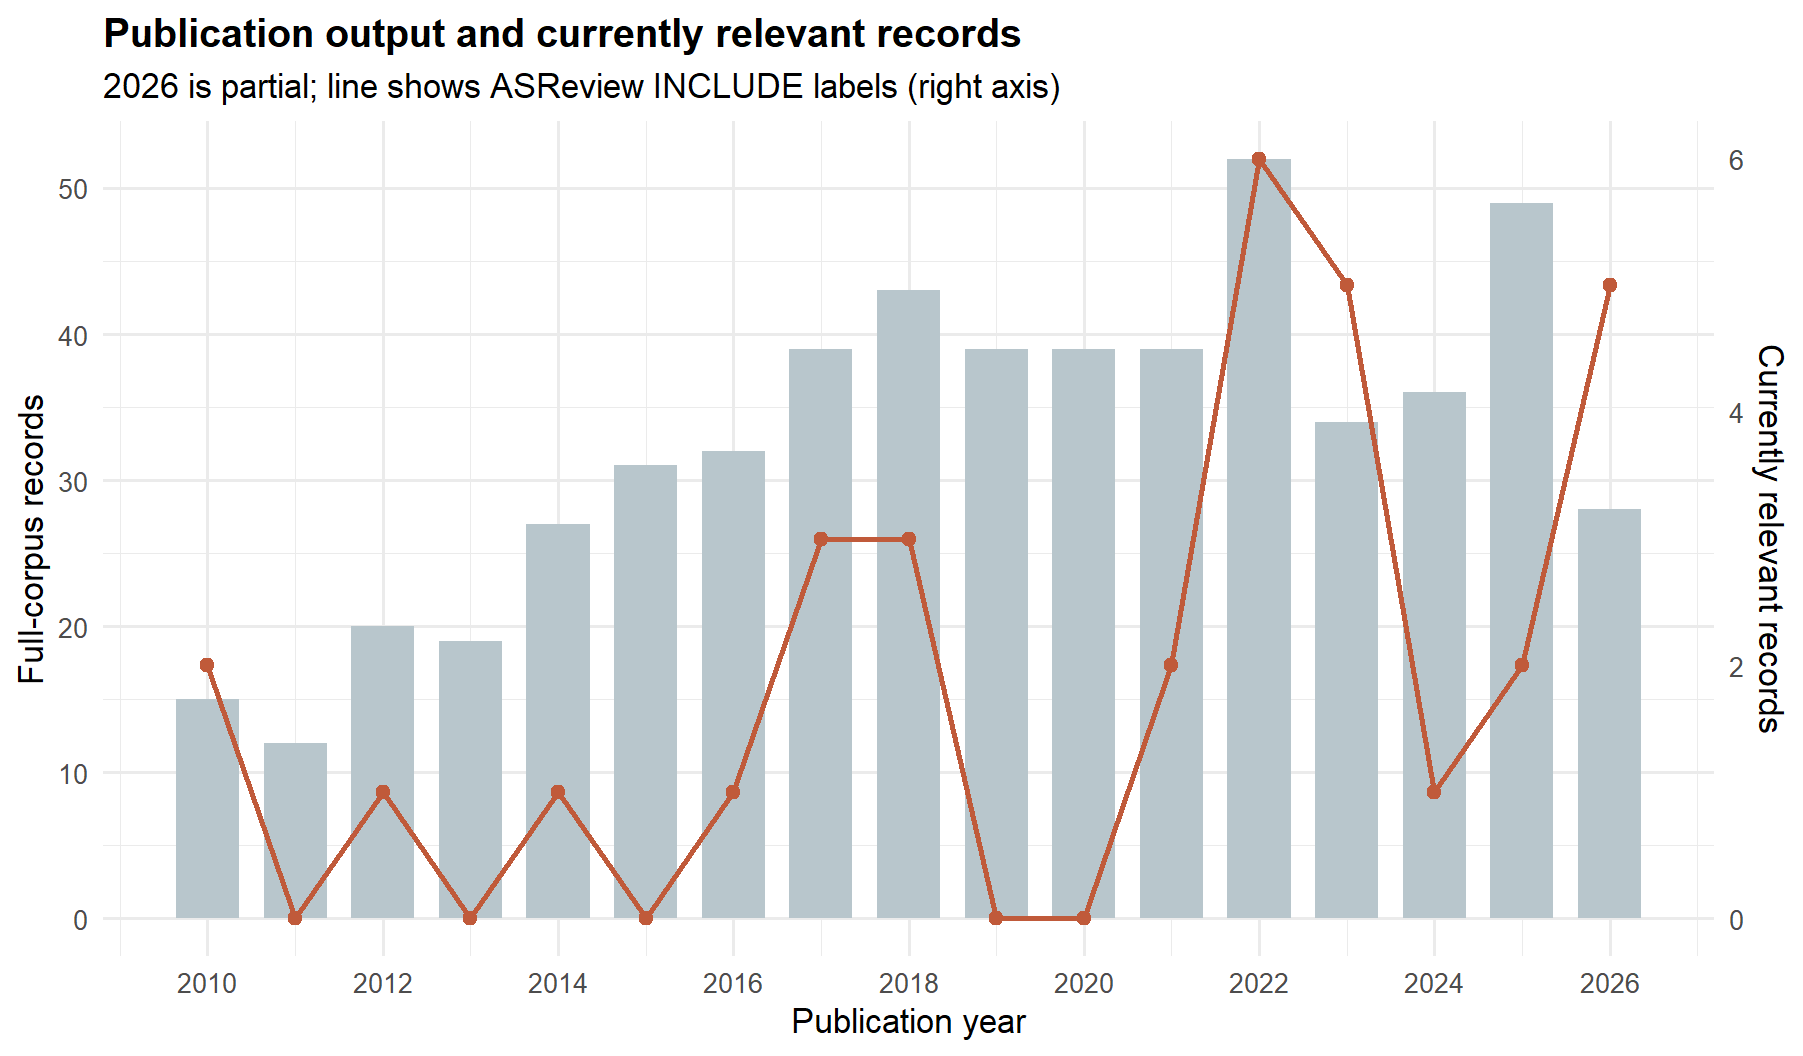
\includegraphics[width=0.88\textwidth]{bibliometrics/annual_production.png}
\caption{Annual publication output in the 554-record corpus and records
currently labeled relevant. The 2026 count is partial.}
\label{fig:annual}
\end{figure*}

\begin{figure*}[!t]
\centering
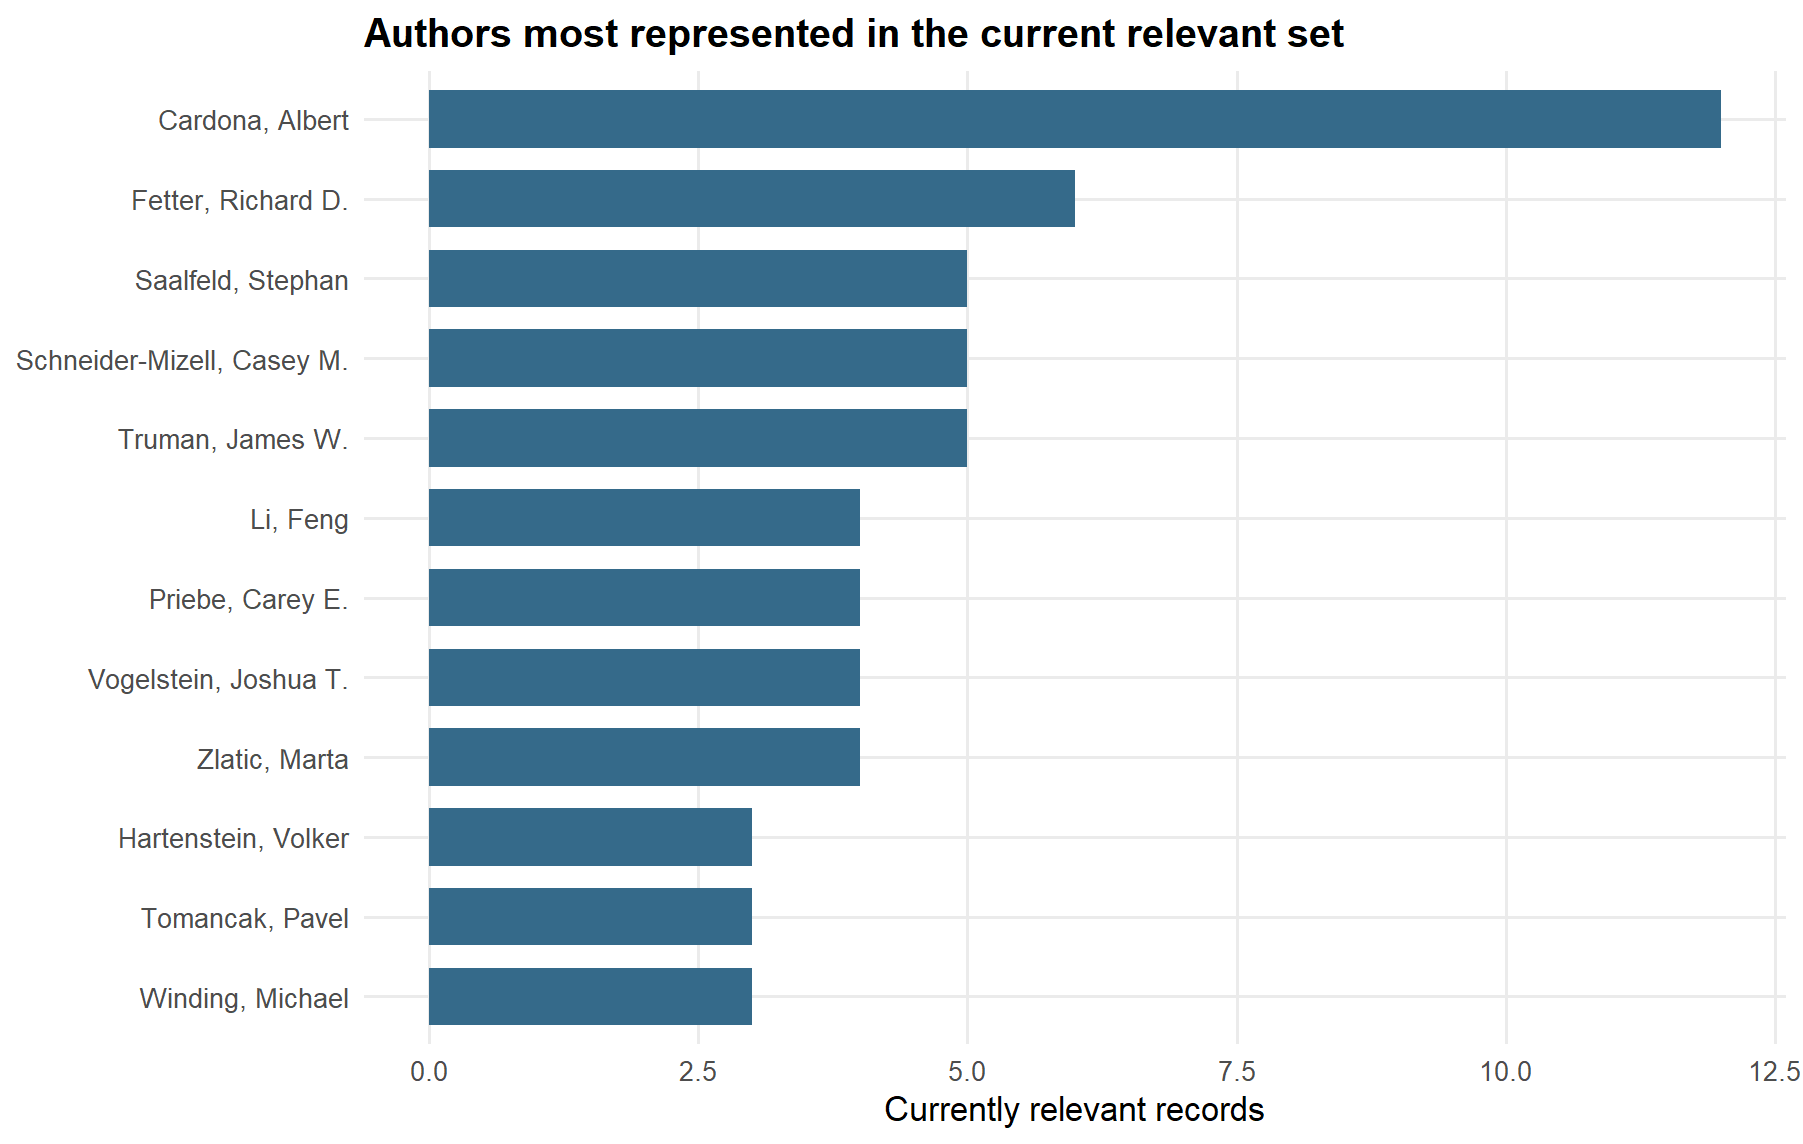
\includegraphics[width=0.78\textwidth]{bibliometrics/authors.png}
\caption{Most frequently listed authors among records currently labeled
relevant.}
\label{fig:authors}
\end{figure*}

\begin{figure*}[!t]
\centering
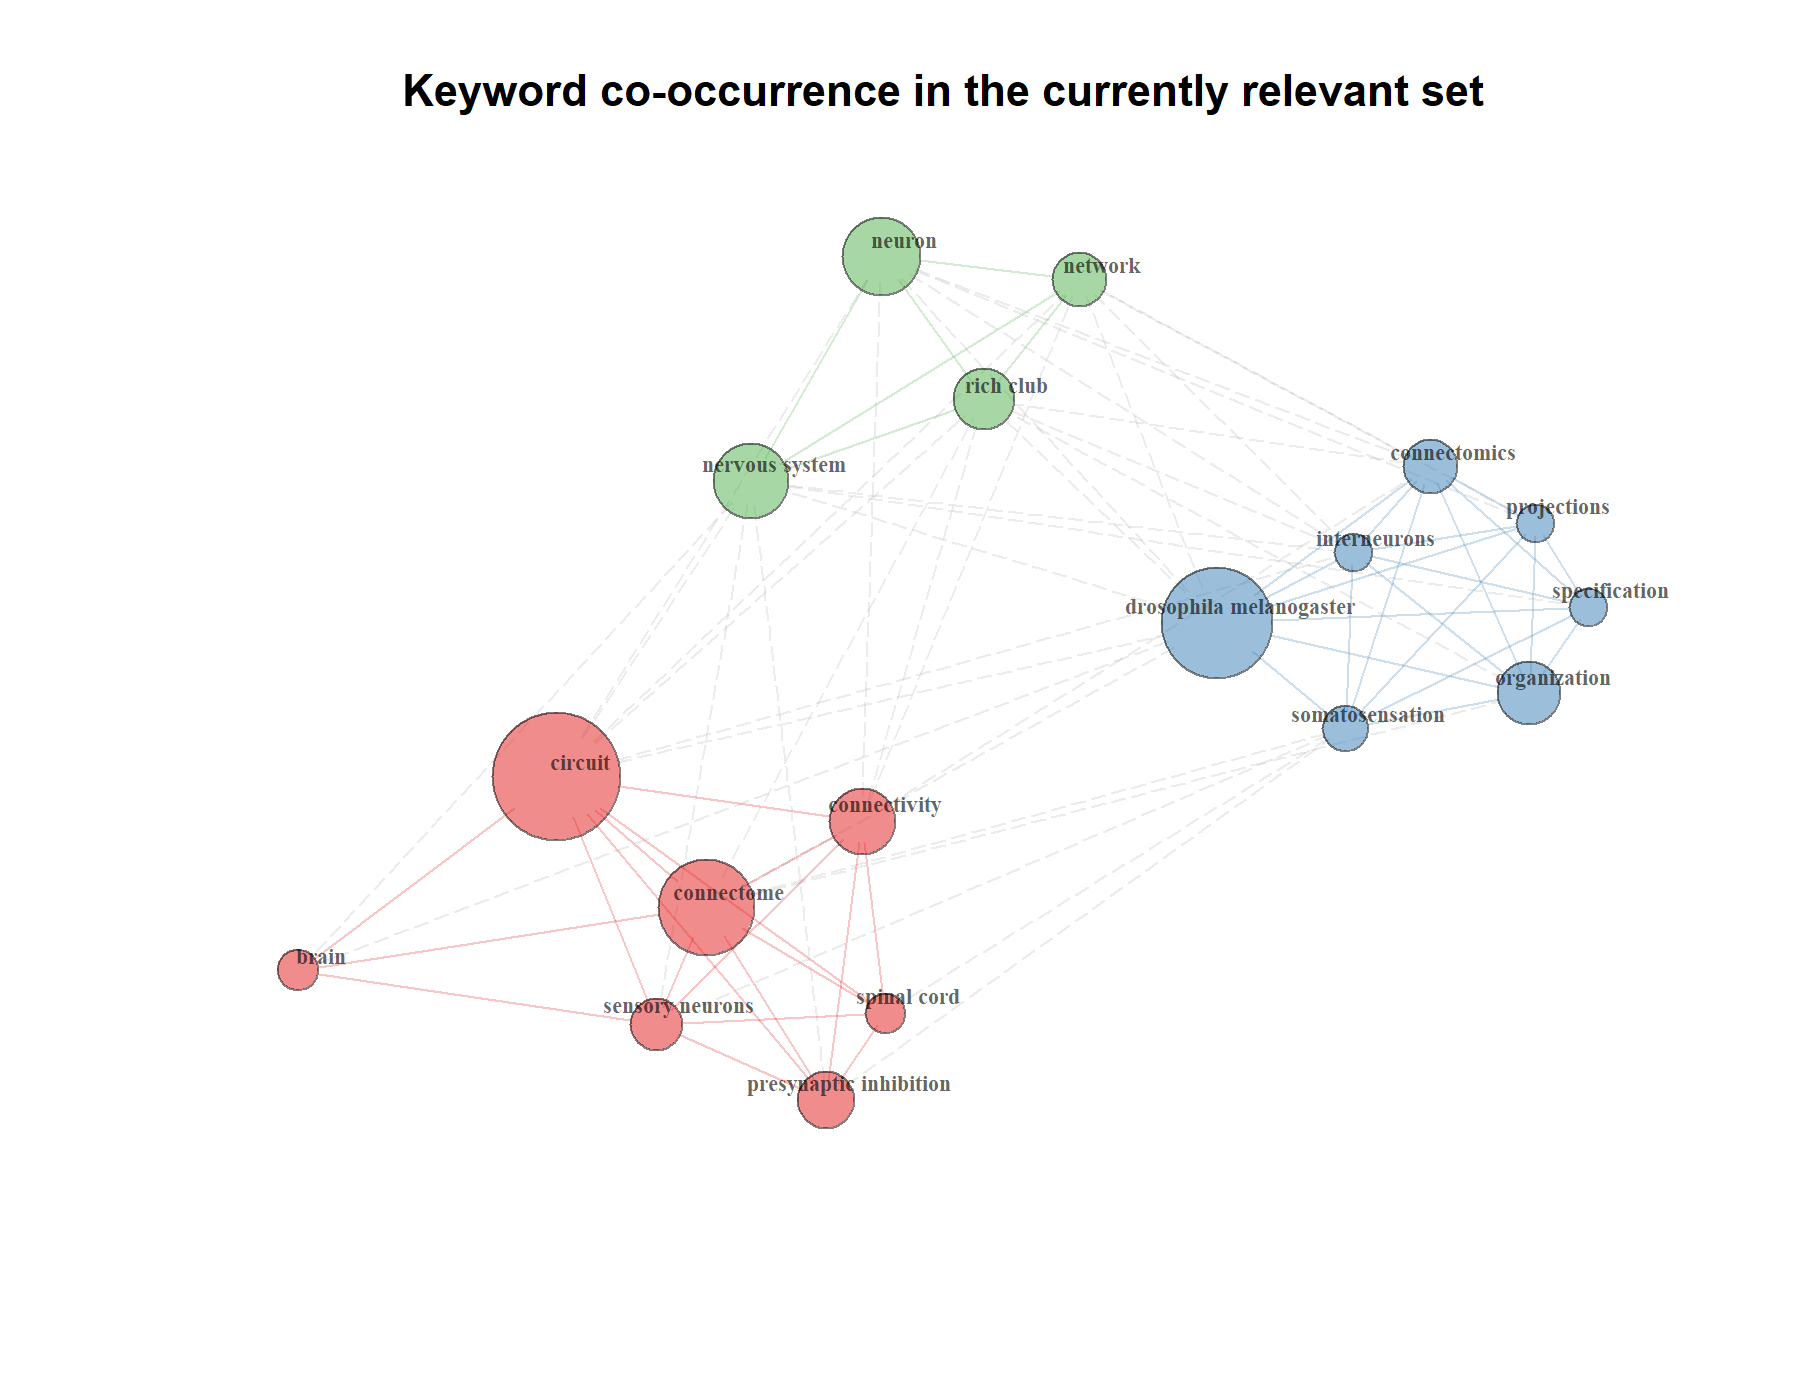
\includegraphics[width=0.78\textwidth]{bibliometrics/keyword_network.png}
\caption{Exploratory co-occurrence network of normalized keyword fields in
the records currently labeled relevant.}
\label{fig:keyword-network}
\end{figure*}

\begin{figure*}[!t]
\centering
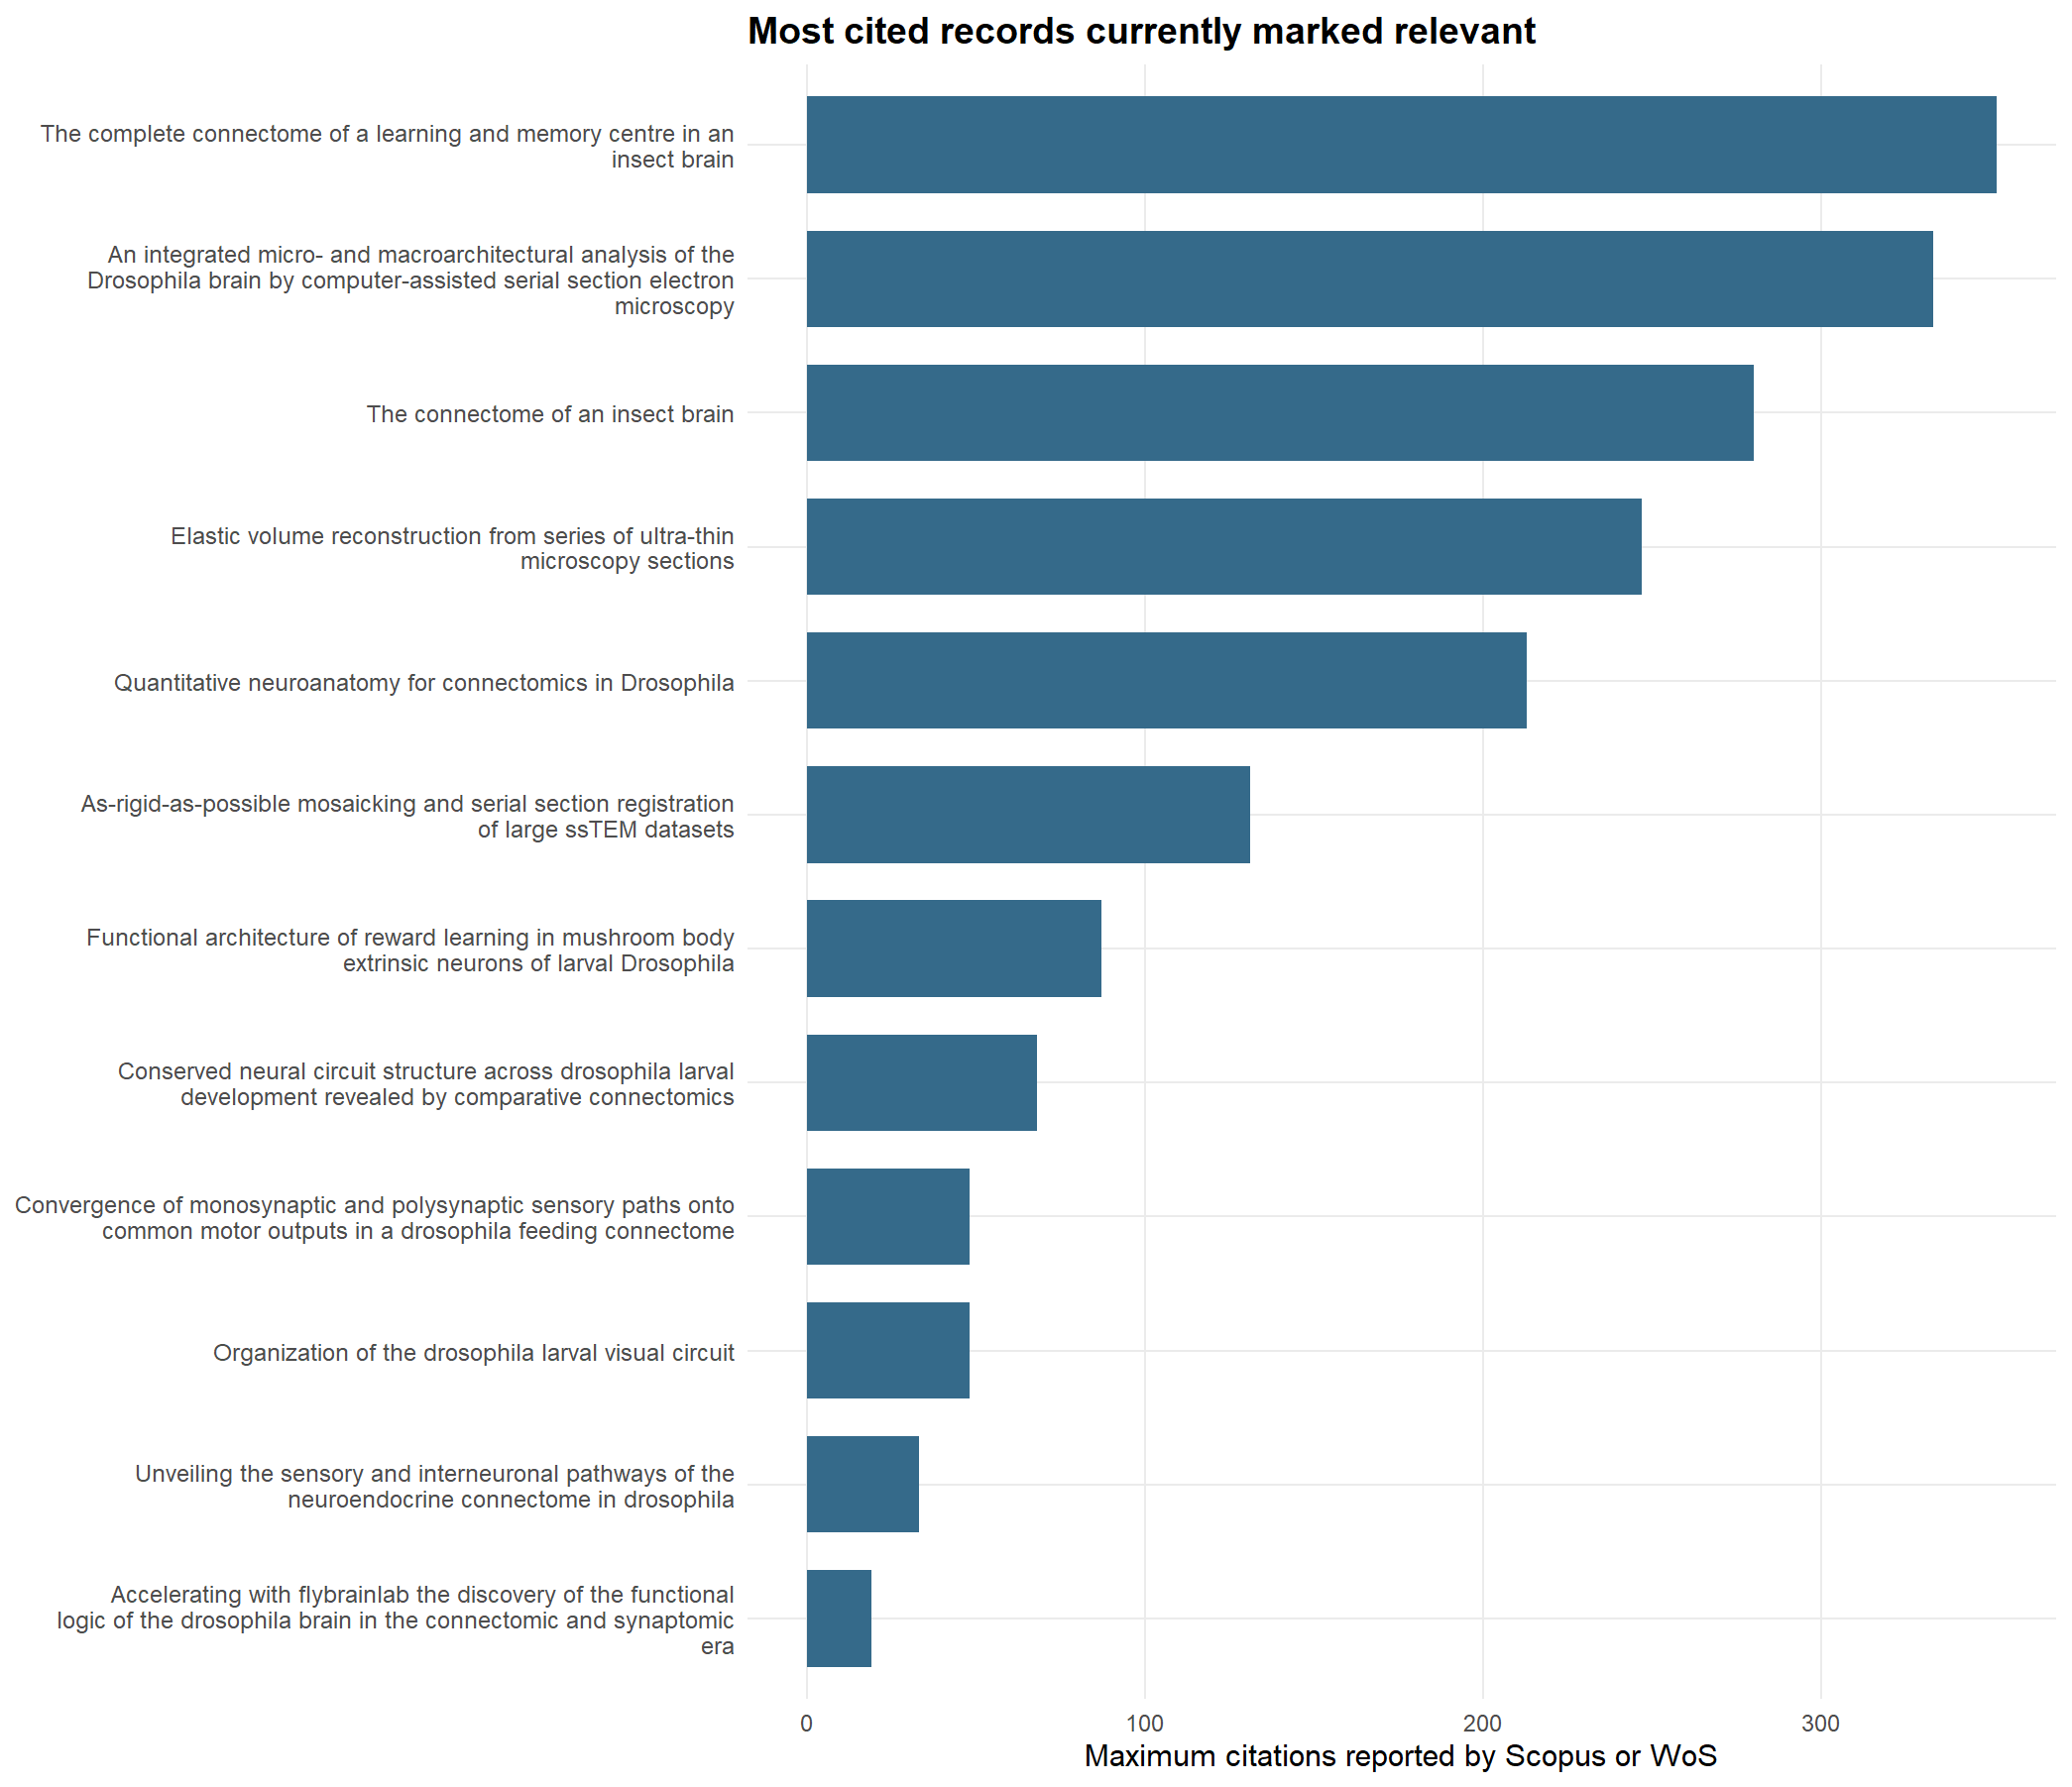
\includegraphics[width=0.82\textwidth]{bibliometrics/citations.png}
\caption{Highest stored citation counts among records currently labeled
relevant. Values are the per-record maximum reported by Scopus or WoS.}
\label{fig:citations}
\end{figure*}

\begin{figure*}[!t]
\centering
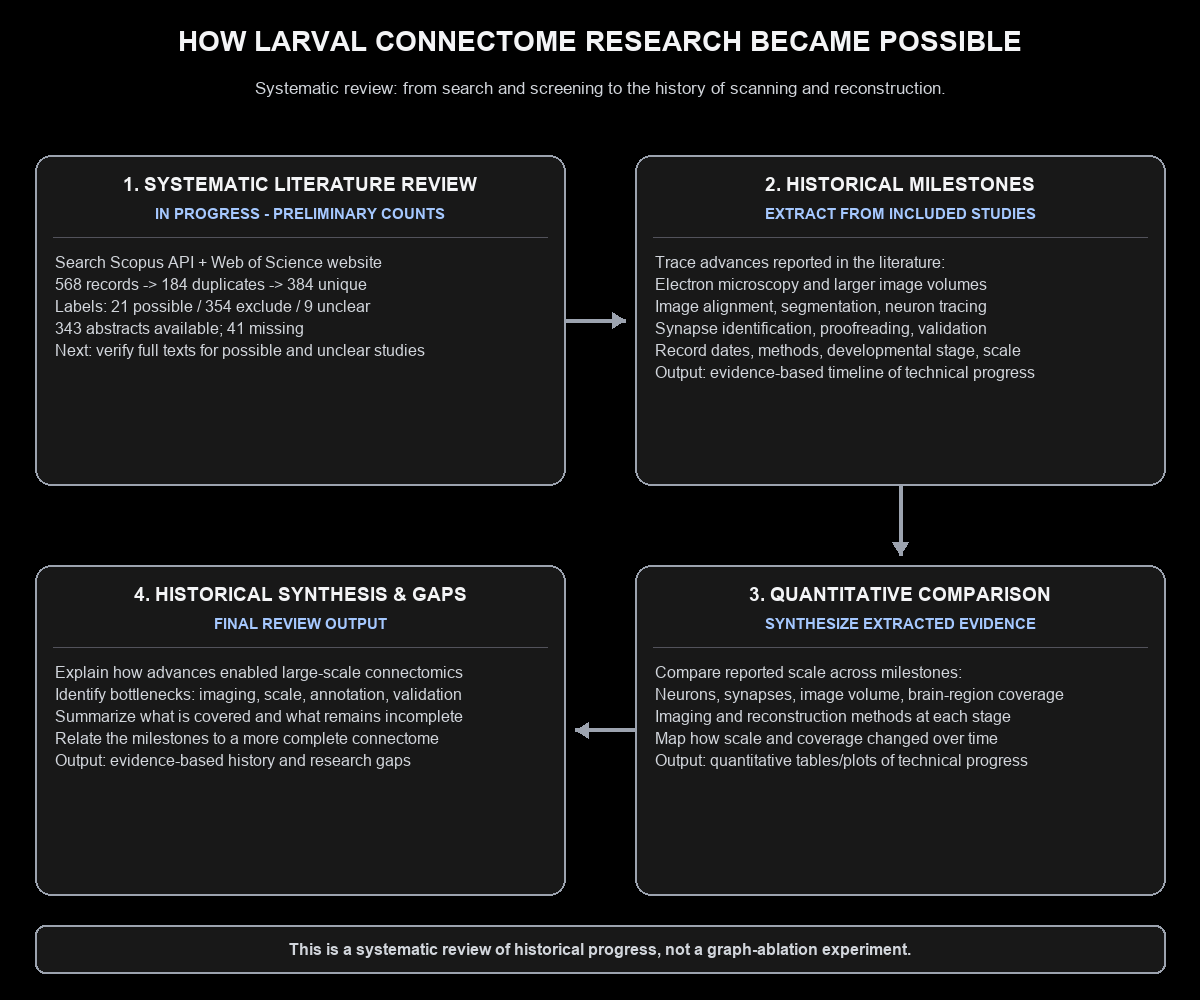
\includegraphics[width=0.95\textwidth]{pipe.png}
\caption{Current progress and planned stages of the historical systematic
review. Screening labels are preliminary; full-text assessment and
historical extraction remain to be completed.}
\label{fig:workflow}
\end{figure*}
